\section{Our Method}
\label{sec:Meth}

 

\begin{figure}[!ht]
	\centering
	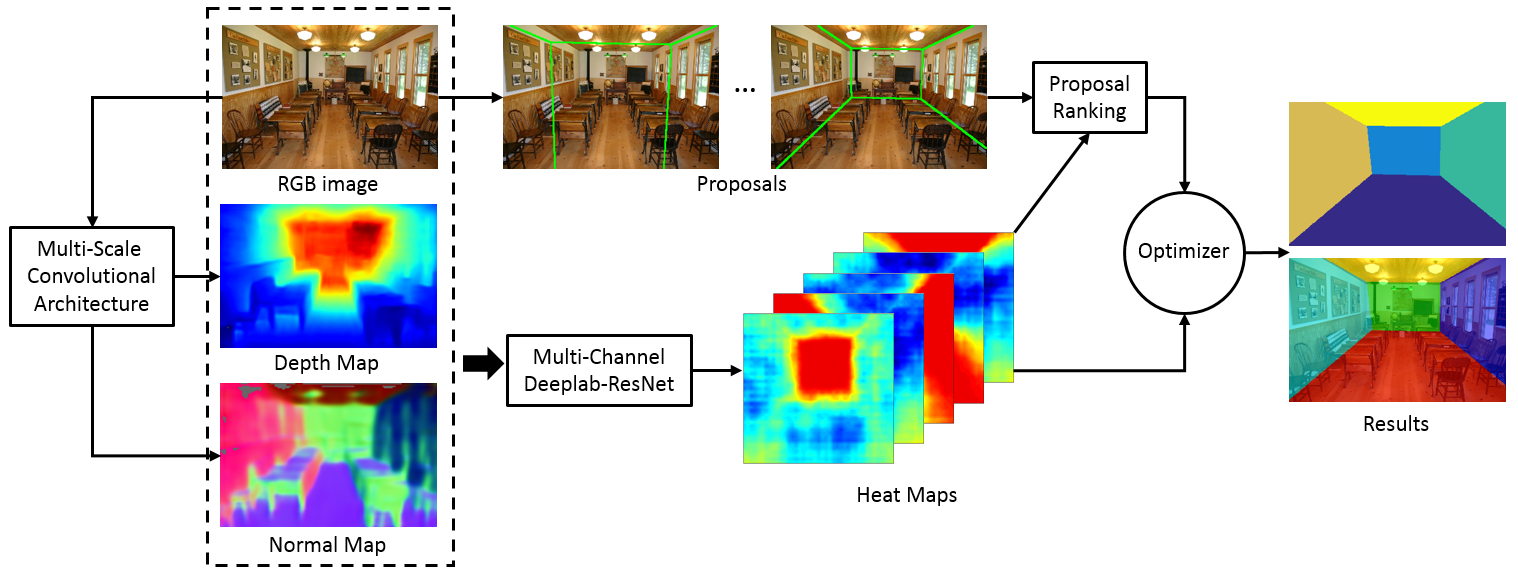
\includegraphics[width=8.5cm]{figure/ppline.png}
	\caption{The pipeline of our layout estimation algorithm. First, we adopt a multi-scale CNN architecture~\cite{eigen2015predicting} to extract the geometric information, including depth and normals, from the RGB image. Then, we combine all the above-mentioned information into a multi-channel FCN, which helps to accurately estimate the layout. Finally, an optimization framework is employed to obtain the final layout by optimizing the best proposals generated from the input RGB image.}
	\label{fig:pipeline}
\end{figure}

Under the Manhattan world assumption \cite{coughlan1999manhattan}, a room layout can be represented as a cube, of which most five surfaces \{Left, Front, Right, Ceiling, Ground\} are visible in an image. 
%
Given an RGB image $\vb{I}$ with an arbitrary size, our algorithm generates a room layout $\vb{L}$ that has a surface label for each pixel $L_{ij}$ in such 5-class set. Fig.~\ref{fig:pipeline} shows the algorithm pipeline. 
%%step 1
We first estimate a depth map $D_{I}$ and a normal map $N_{I}$ from the input image to generate geometric hints, using a multi-scale convolutional network~\cite{eigen2015predicting}, as described in Sec.~\ref{sec:depth_normal}.
%step 2
After that, to integrate the information from the input RGB image together with the geometric hints, a multi-channel fully convolutional network (MC-FCN) is trained. 
The MC-FCN is applied to predict five probability maps, each of which describes the probability of a pixel belonging to a specific layout surface. Details can be found in Sec.~\ref{sec:surfacelabel}.
%step 3: optimization
While we can easily get a layout estimation $\vb{\hat{L}}$ by choosing the label with the highest score among the five probability maps for each pixel, the estimated $\vb{\hat{L}}$ always has wavy boundaries and multiple disjoint connected regions, due to the characteristics of neural networks. 
To handle these problems and obtain clearer layout estimation with geometric constraints, an optimization step is adopted, as described in Sec.~\ref{sec:optimization}.  
 

\subsection{Geometric Hint Extraction}
\label{sec:depth_normal}

We use the multi-scale convolutional network proposed in \cite{eigen2015predicting} to estimate the depth and normal maps from RGB images.
An example is shown in Fig.~\ref{fig:depthandnormal}. 
Note that we do not finetune their models with our data as we do not have the depth and normal data in our dataset.
However, the model seems to generalize well in our case. 
%Quantitative evaluation of their work can be referred to \cite{eigen2015predicting}.
%

\begin{figure}
	\centering
	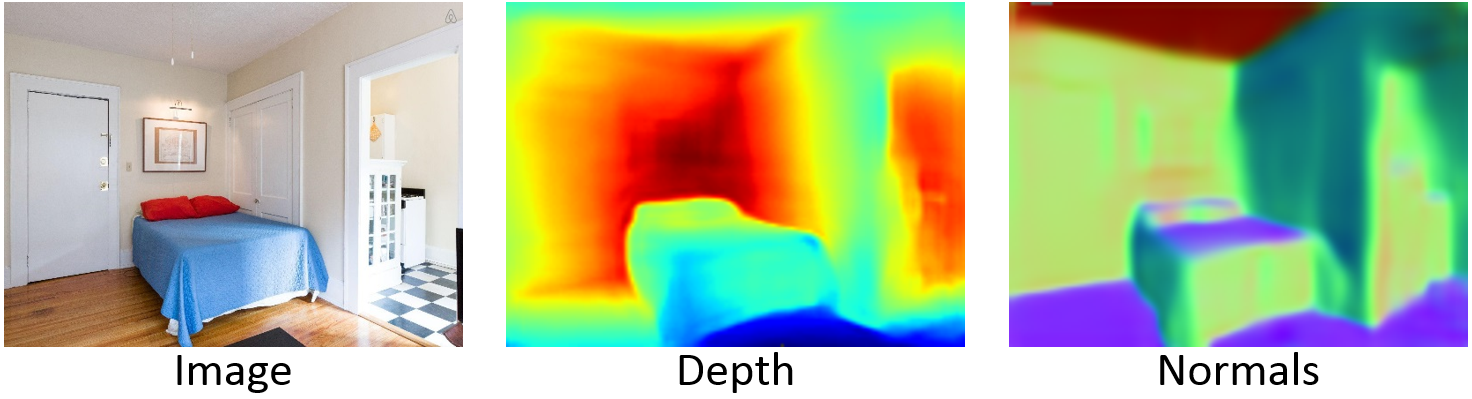
\includegraphics[width=8.5cm]{figure/DN.png}
	\caption{Depths and normals estimated from an RGB image using the multi-scale FCN~\cite{eigen2015predicting}. From the global perspective, the extracted geometric information captures the overall spatial relationships between different surfaces. }
	\label{fig:depthandnormal}
\end{figure}

We notice in practice that the depth and normals estimated from RGB images are not precise in local details. And the output resolution of the depth and normal maps is limited to half of the input. However, the valuable 3D information they provided is much helpful for high-level structure estimation, especially in messy scenes.  
%
As analyzed in Sec.~\ref{sec:ablation}, depths and normals can serve as hints that tend to merge big planes together under the interference factors, such as clutters and occlusions. 
%
Therefore, we apply these mid-level geometric hints to improve the performance of layout estimation. 
%


The depth maps are color coded to 3-channels in \cite{eigen2015predicting} for distinction. In order to ensure the essence of depth and to reduce the redundant information, we modify their rendering section to obtain depth maps with a single channel, which is then fed to the following multi-channel FCN.

\subsection{Semantic Surface Segmentation Using MC-FCN}
\label{sec:surfacelabel}
In prior techniques, FCNs are widely used for semantic surface segmentation \cite{dasgupta2016delay,ren2016coarse,mallya2015learning}. 
%
However, due to clutters, occlusions, complex textures and illumination variations in indoor scenes, the surface segmentation represented as $\vb{\hat{L}}$ is sometimes ruined by irregular spurious regions. 
Fig.~\ref{fig:fcn-comparison} demonstrates several typical inferior cases.
%
To get rid of these annoying spurious regions, we attempt to make our network more robust to miscellaneous environmental factors. 
A multi-channel FCN (MC-FCN) is adopted to incorporate geometric hints that are estimated from the RGB image. 
%


\begin{figure}
	\centering
	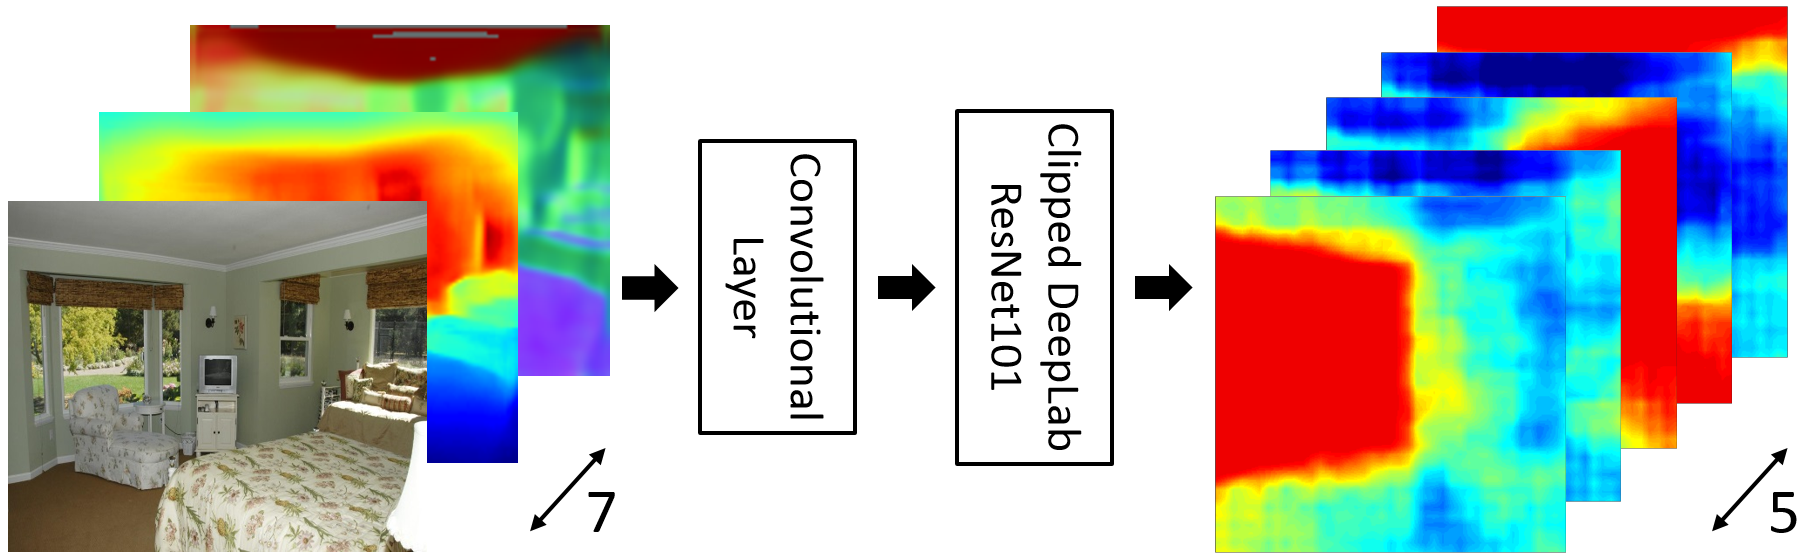
\includegraphics[width=8.5cm]{figure/MC-FCN.png}
	\caption{The multi-channel network architecture build on \cite{chen2016deeplab}. We clip the Deeplab-ResNet101 by removing the multi-scale related layers. Then, we combine the RGB image, depth and normals together as input to the network for semantic surface learning. }
	\label{fig:fcn-multi-channel}
\end{figure}

\vspace{0.1cm}
\noindent\textbf{Network Architecture.}
We build the MC-FCN based on the DeepLab-ResNet101~\cite{chen2016deeplab}. 
%
While we consider the room layout as a high-level semantic information that relies more on global structure, we modify the network by removing the multi-scale related layers. 
As illustrated in Fig.~\ref{fig:fcn-multi-channel}, the estimated depth and normal maps are treated as additional channels associated with the input RGB image. 
We simply concatenate different types of data to a seven-channels input (3 channels from RGB, 1 channel from depth and 3 channels from normals), and feed them into the network. 
Atrous convolution is adopted in our 5-way classifier layer. 

\vspace{0.1cm}
\noindent\textbf{Training.} We initialize the MC-FCN parameters with a model pre-trained on the SUNRGBD dataset, except for the classifier layer. 
After that, the MC-FCN is specifically fine-tuned for semantic surface segmentation.
%
The output of our MC-FCN is a $w\times h \times 5$ probability array $\vb{T}$, where $w$ and $h$ stand for the width and length of the input image. Each of the 5 slices can be viewd as a probability map for the corresponding surface label, as shown in Fig.~\ref{fig:fcn-multi-channel}. We utilize the probability array $\vb{T}$ as the basis for our scoring function in the proposal ranking and optimization step. 
 


\begin{figure}
	\centering
	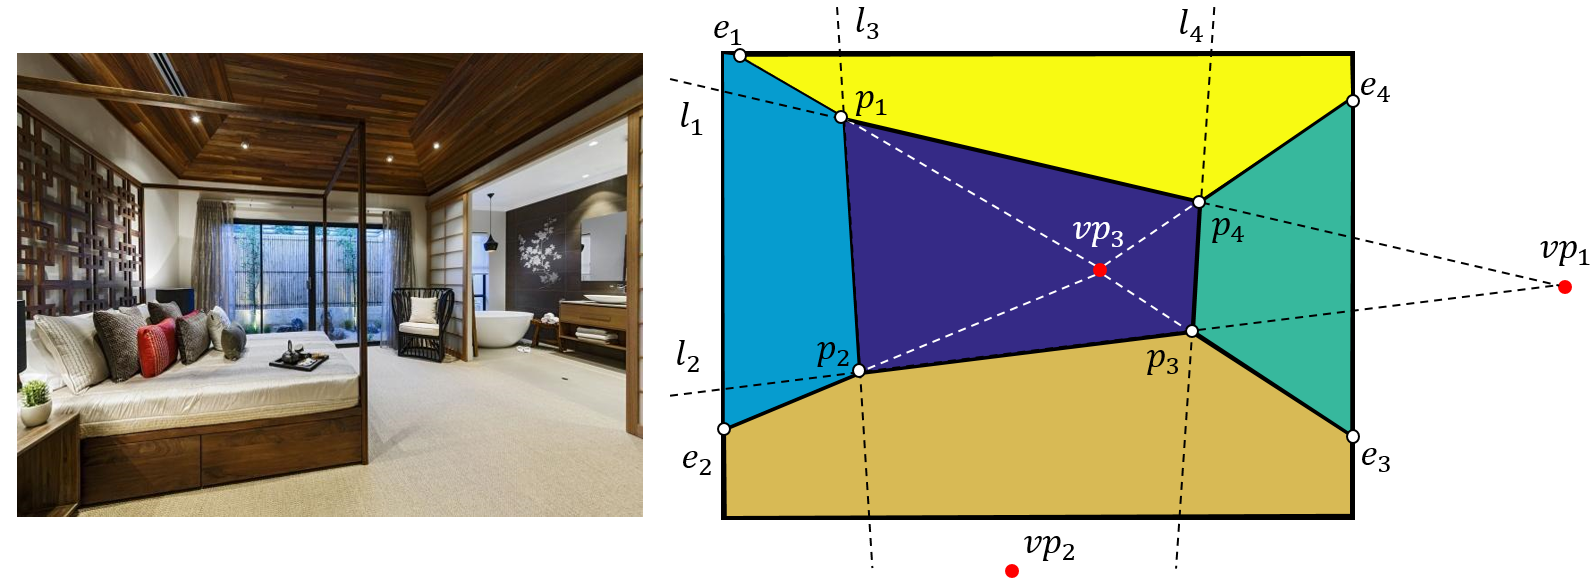
\includegraphics[width=8.5cm]{figure/parameterization.png}
	\caption{ Illustration of the parameterized model $\tau$. The vanishing points $vp_1$ and $vp_2$ are applied for extracting proposals. }
	\label{fig:parameterization}
\end{figure}


\subsection{Layout Optimization}
\label{sec:optimization}
We adopt a widely used model~\cite{hedau2009recovering, wang2013discriminative, dasgupta2016delay, ren2016coarse} to parameterize an indoor layout based on the Manhattan world assumption. A scene layout is modeled as the projection of a cuboid, which can be defined by 

\begin{equation}
	\label{eq:Layout}
	\tau = (l_1, l_2, l_3, l_4, vp_3),
\end{equation}
%
where $l_{i}$ stands for the $i^{th}$ line and $vp_3$ stands for the vanishing point near the image center, as illustrated in Fig.~\ref{fig:parameterization}.
%
Dasgupta et al.~\cite{dasgupta2016delay} proposed an iterative refinement algorithm to obtain a precise layout. 
They directly take $\vb{\hat{L}}$ as initialization and process it to address spurious regions and multiple disjoint components. 
However, as mentioned above, the initial $\vb{\hat{L}}$ generated from $\vb{T}$ is often too ambiguous due to the characteristics of neural networks.
The preprocessing step can not adapt to all the misleading situations, especially when the sizes of ambiguous walls are similar. 
%%

To make the optimization method more general and efficient, we simplify the refinement algorithm in \cite{dasgupta2016delay} by replacing the initialization and preprocessing step with a proposing-ranking framework. The framework directly generates the initial $\vb{L^*}$ consistent with the formulation in Eq.~\ref{eq:Layout}. This kind of $\vb{L^*}$ is much robust to ambiguous cases and easier for the optimization step to find the best layout.

Our proposing-ranking framework is similar with \cite{hedau2009recovering}.
The score function is constructed based on the surface prediction $\vb{T}$. 
At first, straight lines are found and grouped to detect three vanishing points. 
Then, we sample 30 rays from $vp_1$ and $vp_2$ respectively to acquire numerous proposals, each of which is specified by two rays from each vanishing point. Finally, for any given proposal $\vb{\overline{L}}$ with $r$ semantic surfaces, we define the score function as:
%
\begin{equation}
\label{eq:scorefunction}
S(\vb{\overline{L}}~|~\vb{T}) = \frac{1}{w\times h}\sum_r \vb{T}_r^{(\overline{L}_r)},
\end{equation}
%
where $r$ represents the pixels in a certain region for the corresponding semantic surface. Intuitively, the proposal with higher score is more similar to $\vb{\hat{L}}$ and also conforms to geometric projection constraints. We select the proposal with the highest score as initial $\vb{L^*}$, namely:
%
\begin{equation}
\label{eq:initial}
\vb{L^*} = \arg\max_{\vb{\overline{L}}} S(\vb{\overline{L}}~|~\vb{T}).
\end{equation}
%
After the proposing-ranking framework, $\vb{L^*}$ is further refined to attain precise $\vb{L}$ using the optimization step in \cite{dasgupta2016delay}.

\comments{
(deleted)We further modify the score function and apply it to the following optimization step:
%
\begin{equation}
\label{eq:optimize}
S(\vb{L}~|~\vb{T}) = \frac{1}{wh}\sum_{r} \vb{T}_{r}^{L_{r}} + \frac{1}{wh}\sum_{r^*} \arg\max_{L_{r^*}} \vb{T}_{r^*}^{L_{r^*}}
\end{equation}
%
Where $r \in$ \{Ceiling, Floor\} and $r^* \in$ \{Left, Front, Right\}. The second term including an argmax operation is designed for three walls. As shown in Fig.~\ref{fig:parameterization}(a), there is an inherent ambiguity between front wall and right/left wall. While Dasgupta et al. \cite{dasgupta2016delay} treat it as a special case, our score function cope with the ambiguity generally.}

